\documentclass[10pt]{beamer}

\usetheme[progressbar=frametitle]{metropolis}
\usepackage{appendixnumberbeamer}
\usepackage[utf8]{inputenc}    
\usepackage{booktabs}
\usepackage[scale=2]{ccicons}

\usepackage{pgfplots}
\usepgfplotslibrary{dateplot}

\usepackage{xspace}
\newcommand{\themename}{\textbf{\textsc{metropolis}}\xspace}

\title{Porovnanie typov rekurentných neurónových sietí z hľadiska hĺbky pamäte}
\subtitle{Diplomová práca}
% \date{\today}
\date{}
\author{Jaroslav Ištok}
%\institute{Faculty of Mathematics Physics and Informatics Comenius University Bratislava}
% \titlegraphic{\hfill\includegraphics[height=1.5cm]{logo.pdf}}

\begin{document}

\maketitle

\begin{frame}{Obsah}
  \setbeamertemplate{section in toc}[sections numbered]
  \tableofcontents[hideallsubsections]
\end{frame}

\section{Implementácia}
\begin{frame}[fragile]{SOM}

\begin{itemize}
  \item samoorganizujúca sa mapa
  \item biologicky motivovaný model
  \item učenie so súťažením
  \item učenie bez učiteľa
  \item zhlukovanie dát
  \item zachovanie topologických vlastností dát
\end{itemize}

Hľadanie víťaza
\begin{equation*}
i^* = argmin_i||x-w_i|| 
\end{equation*}

Aktualizácia váh
\begin{equation*}
w_i(t+1) = w_i(t) + \alpha(t)h(i^*, i)([x(t) - w_i(t)]
\end{equation*}

\end{frame}


\section{Elmanova rekurentná neurónová sieť}

\begin{frame}[fragile]{Elmanova rekurentná neurónová sieť}
\begin{itemize}
\item Učenie s učiteľom 
\item Trénovanie pomocou algoritmu spätného šírenia chyby cez čas
\item Kontextová vrstva neurónov (kontextové neuróny)
\end{itemize}
\end{frame}

\begin{frame}[fragile]{Elmanova rekurentná neurónová sieť}

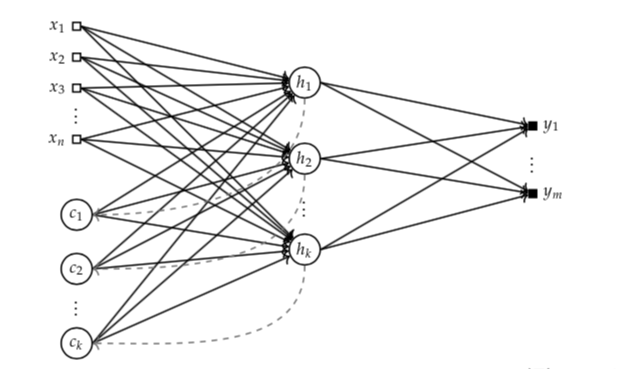
\includegraphics[width=\textwidth]{elman}

\end{frame}


\section{Rekurentná SOM}

\begin{frame}[fragile]{Rekurentná SOM}
Je to samoorganizujúca sa mapa, 
\begin{itemize}
\item RecSom - kontextom je kópia mapy z predchádzajúceho kroku
\item Veľké množstvo atribútov
\end{itemize}
Aktualizácia váh
\begin{equation*}
w_i(t+1) = w_i(t) + zh_{ik}[s(t) - w_i(t)]
\end{equation*}
\begin{equation*}
c_i(t+1) = c_i(t) + zh_{ik}[y(t - 1) - c_i(t)]
\end{equation*}
\begin{equation*}
y_i=exp(-d_i)
\end{equation*}
Vzdialenosť
\begin{equation*}
d_i(t) = \alpha||x(t)-w_i||^2 + \beta||r(t)-c_i||^2
\end{equation*}
Rekurzívny kontext
\begin{equation*}
r(t)=[y_i(t-1),...,y_N(t-1)]
\end{equation*}
\end{frame}

\section{Merge SOM}

\begin{frame}[fragile]{Merge SOM}

\begin{itemize}
\item V merge SOM kontext nie je kópia celej mapy z predchádzajúceho kroku
\item Kontextom je iba stav víťazného neurónu z predchádzajúceho kroku
\item Menej parametrov ako pri rekurzívnej SOM
\item $\gamma_1$ $\gamma_2$ - parametre rýchlosti učenia
\item $h_{\sigma}$ - excitačná funkcia
\item $d_N$ - susedná funkcia
\end{itemize}
Aktualizácia váh
\begin{equation*}
\Delta w_i = \gamma_{1} \cdot h_{\sigma}(d_{N}(i, I_{t})) \cdot (x^t - w^i)
\end{equation*}
\begin{equation*}
\Delta c_i = \gamma_{2} \cdot h_{\sigma}(d_{N}(i, I_{t})) \cdot (c^t - c^i)
\end{equation*}

Vzdialenosť
\begin{equation*}
d_i(t) = (1-\alpha) \cdot ||x^t - w^i||^2 + \alpha \cdot ||c^t - c^i||^2
\end{equation*}

Rekurzívny kontext
\begin{equation*}
c^t = (1 - \beta) \cdot w^{I_{t-1}} + \beta \cdot c^{I_{t-1}}
\end{equation*}
\end{frame}

\begin{frame}[fragile]{Meranie pamäťovej hĺbky}

\begin{itemize}
\item sekvencie slov
\item každý neurón má množinu písmen
\item tieto tvoria tzv. receptívne pole neurónovej siete
\item každý neurón si zapamätá $k$ posledných znakov
\item nájdeme najdlhšiu spoločnú podpostupnosť pre každý neurón
\item tým získame pamäťovú hĺbku pre jednotlivé neuróny
\item ked spravíme výhovaný priemer pamäťových hĺbok pre všetky neuróny v sieti dostaneme pamäťovú hĺbku pre celú sieť
\item toto číslo budeme používať ako mieru pamäťovej hĺbky pre SOM
\end{itemize}

\end{frame}

\begin{frame}[fragile]{Ukážka receptívneho poľa}
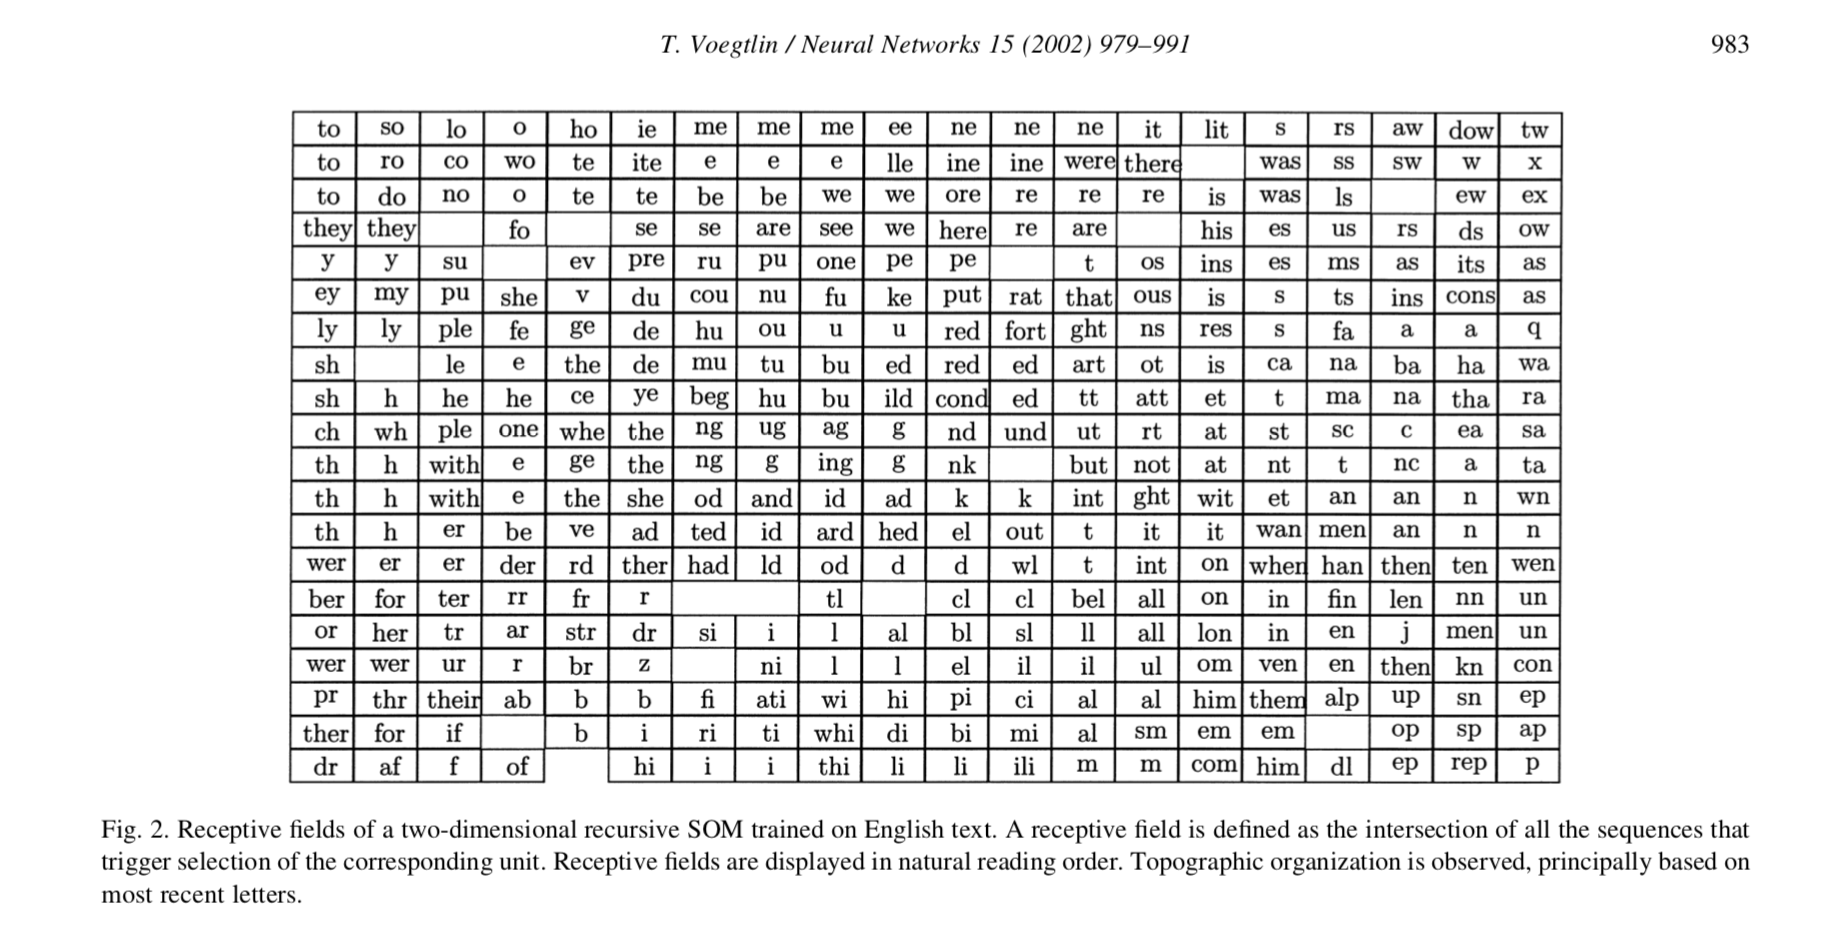
\includegraphics[width=\textwidth]{receptive_field}
\end{frame}

\begin{frame}{Implementácia}

\begin{itemize}
  \item Vlasná implementácia sietí
\end{itemize}

\end{frame}


{\setbeamercolor{palette primary}{fg=black, bg=yellow}
\begin{frame}[standout]
  Otázky
\end{frame}
}

\appendix


\begin{frame}[allowframebreaks]{References}

  \bibliographystyle{abbrv}
  
\begin{thebibliography}{9}
\bibitem{srn} 
Jeffrey L.Elman
\textit{Finding Structure in Time}. 
University of California, San Diego, 1990
 
\bibitem{som} 
H. Ritter and T. Kohonen
\textit{Self-Organizing Semantic Maps} 
Helsinky University of Technology, 1982
  
\bibitem{recsom} 
Thomas Voegtlin
\textit{Recursive self-organizing maps}, 2002
 
\bibitem{msom} 
Marc Strickert, Barbara Hammer
\textit{Merge SOM for temporal data}
Technical University of Clausthal, 2005
 
\end{thebibliography}

\end{frame}

\end{document}
